\lab{Python}{Optimization with Scipy}{scipy.optimize}
\label{lab:Optimization1}
\objective{Introduce some of the basic optimization functions available in \li{scipy.optimize}}

The Optimize package in Scipy has several types of optimizing algorithms.
This lab will introduce some of the basic types of algorithms included.

You can learn about all of the functions at \url{http://docs.scipy.org/doc/scipy/reference/optimize.html}.


Last week, a word reached your village that the dread pirate Roberts buried some treasure at the lowest point of a nearby valley.
$5$ men immediately prepared to reclaim the treasure.
Afraid of the competition, they each asked the village sage for advice on how to reach the treasure faster than the others.
Deciding that the pursuit of knowledge was more important than gold, the sage conducted an experiment on the men.
Each man was given a different formula to reach the bottom.  

The algorithms were 
\begin{itemize}
\item Downhill Simplex
\item Conjugate Gradient
\item BFGS
\item Modified Powell
\item Newton Conjugate Gradient
\end{itemize}

You may recognize some of these algorithms, and several of them will be discussed in greater detail later.
For this lab, you do not need to understand how they work.


The valley, seen in the topographical Figure \ref{opt:rosenbrock}, is represented by the Rosenbrock Function, which satisfies the equation $f(x,y) = (1-x)^2 + 100(y-x^2)^2$.
The Rosenbrock fuction is a common optimization algorithm checking function, so it is included in the optimize package.
You can either define or import it.
Note that for some algorithms, you'll need the gradient and/or hessian.

\begin{figure}
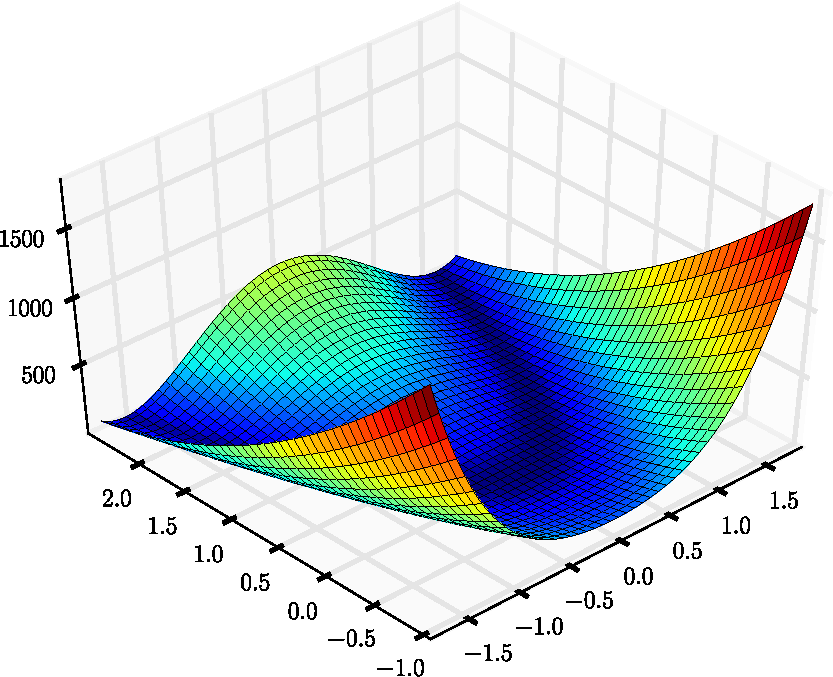
\includegraphics[width=\textwidth]{Rosenbrock.pdf}
\caption{$f(x,y) = (1-x)^2 + 100(y-x^2)^2$}
\label{opt:rosenbrock}
\end{figure}

Use the scipy optimize package to answer the following questions:

\begin{itemize}

\item Where is the treasure buried?

\item In which order did they reach the treasure? Was this consistent from each $x_0$.

\item Where there any men who didn't reach treasure?

\end{itemize}

Group 1: Nelder-Mead Simplex
In Python

\begin{lstlisting}[style=python]
>>> def rosen(x):
	return sum(100.0*(x[1:]-x[:-1]**2.0)**2.0 + (1-x[:-1])**2.0))

>>> x0 = np.array([1.3, 0.7, 0.8, 1.9, 1.2])
>>> res = minimize(rosen, x0, method='nelder-mead', options={'xtol': 1e-8, 'disp': True})

Group 2

Group 3

Group 4
\end{lstlisting}
